I start with a brief review of useful concepts to go trough Kittel's book

\subsection*{General information about waves}
Let us consider the wave equation 
\begin{equation*}
    \frac{\partial^2u(x,t)}{\partial x^2} = \frac{1}{v^2} \frac{\partial^2u(x,t)}{\partial t^2}
\end{equation*}
One solution is the function 
\begin{equation}
    u(x,t) = Ae^{i(kx - \omega t)}
    \label{eq:waveeq_solution}
\end{equation}
where $k$ and $\omega$ are two numbers such that $v^2 = \omega^2 / k^2$ and the minus sign at the exponent is purely conventional. \\
One first important consideration is that 
\begin{equation*}
    u(x-vt,0) = Ae^{i(kx - kvt)} = Ae^{i(kx - \omega t)} = u(x, t)
\end{equation*}
this means that the value of the function $u$ at position $x$ at time $t$ is equal to the value of the function $t$ seconds before, in a position
traslated from $x$ to the same distance that a particle with velocity $v$ would cover in the time $t$. In other words, these types of solutions
are rigid waves that traslates in time and space without deforming with velocity $v$. If at time $t$ the point of a wave is at position $x_1$ where do we find it 
at time $t_2 = t+t_0$? From what just said the same point will be at position $x(t_2) = x(t) + vt_0$. In general a wave point motion equation is $x(t) = x(0) + vt = x(0) + \frac{\omega}{k}t)$ so it moves
with a velocity $v$ (called \emph{phase velocity}). \\ 
Since the wave equation is a linear equation (derivatives do not "mix"), a linear combination of functions of the previous form is 
still a solution. Hence, chosen $k_1, \dots, k_N$ and $\omega_1, \dots, \omega_n$ such that $\omega_i/k_i = v$, the function 
\begin{equation*}
    u(x,t) = \sum_{n=1}^N A(k_n) e^{i(k_nx - \omega(k_n) t)}
\end{equation*}
is still a solution of the equation (can be verified by direct subsitution and imposing polynomials identity).
In particular we can take a "continous" linear combination such that 
\begin{equation}
    u(x,t) = \int_{-\infty}^{+\infty} A(k) e^{i(kx - \omega(k)t)} \, dk
    \label{eq:waves_superposition}
\end{equation}
This function can be viewed as the Fouries transform of a function $u(k,t) = A(k)e^{ikx}$.
Every function (wave) $A(k)$ sufficiently regular can be written in terms of a linear combination of sines and cosines (indeformable waves). \\
Now suppose that $A(k)$ is peaked around a value $k_0$ so that we can expand $\omega(k)$ at first order 
$$\omega(k) \simeq \omega(k_0) + \frac{d\omega(k)}{dk}(k-k_0)$$ Equaton \ref{eq:waves_superposition} can be rewritten as 
\begin{equation*}
    u(x,y) \simeq A(k_0)e^{i(k_0x - w(k_0) t)} \int_{-\infty}^{+\infty} e^{i(\omega'(k)(k-k_0))t} \, dk 
    \equiv f(x,t) \cdot g(t)
\end{equation*}
The first factor $f(x,t) = A(k_0)e^{i(k_0x - w(k_0) t)}$ is a plane wave with phase velocity $\omega_0 \equiv \omega(k_0)$, while the second factor
$g(t) = \int_{-\infty}^{+\infty} e^{i(\omega'(k)(k-k_0))t} \, dk$ modulates the wave in time as an envelope that moves with velocity $\omega'(k)$, called the \emph{group velocity}.

\subsection*{Phonons and quantization}
\subsubsection*{Phonons}
Let us consider a lattice with monoatomic base. The force acting on the $n-th$ atom in the chain is 
$$F_n = C\left(x_{n+1} + x_{n-1} - 2 x_n\right)$$
where $x_k$ indicates the displacement of the $k-th$ particle with respect to its equilibrium position. \\
We are interested in solutions of the type 
\begin{equation*}
    x_n(t) = A \exp\left(i(nka - \omega_n t)\right)
\end{equation*}
that is waves of the form as in \ref{eq:waveeq_solution}. By popping this expression into the Newton motion equation for the $n-th$ particle,
we get out that in order to satisfy the equality the following relation must hold
\begin{equation*}
    \omega(k) = 2\sqrt{\frac{C}{M}} \ \left|\sin\left(\frac{ka}{2}\right)\right|
\end{equation*}
this is called the \emph{dispersion relation} and (intuitively) indicates the relationship between the time periodicity ($\omega$) and space periodicity ($k$). \\
For $|k| < \pi/a$ we say that we are in the Brillouin zone of the crystal: the border's values $k=\pm \pi/a$ represents the maximum value for $\omega(k)$ and between 
this range all possible values of $\omega(k)$ are covered: in fact it is easy to see that $\omega(k) = \omega(2k+N\pi/a), \ N \in \mathbf{N}$ (see plots on Kittel for better intuition). Remeber that
$2N\pi/a$ is a reciprocal lattice vector! The particualr significance of the borders of the Brillouin zone is that the wave is standing: there is no space dependence (we wil examin this point later better, but for a visual 
understanding see https://www.khanacademy.org/science/high-school-physics/waves-and-sound/standing-waves-2/v/standing-waves-on-strings). Just note that in this case 
$x_n(t) = (-1)^n \ A \exp(i \omega_0 t)$ and $$x_{n+1}(t)/x_n(t) = -1$$ or, in other words, each atom moves in the opposite direction of the one before: this implies that the center of mass of the chain stays fixed
(and explains why phonons do not carry physical momentum).

\subsubsection*{Quantization}
Let us consider an infinitesimal volume $dV$ centered in $\ve{r}$ of a monoatomic crystal and let us consider a standing wave of the type 
\begin{equation}
    u(t) = u_0 \cos(kx)\cos(\omega t)
    \label{eq:continuous_displacement}
\end{equation}
Stationarity requires that $nKa = \pi$ where $a$ is the lattice constant. \\
Now let us use the quantum virial theorem to calculate
\begin{equation*}
    \left(n + \frac{1}{2}\right) \hbar \omega = \left\langle H \right\rangle = 
    \left\langle T \right\rangle + \left\langle V \right\rangle = 2\left\langle T \right\rangle
    \label{eq:energy_quantization_lattice}
\end{equation*}
To estimate $\left\langle T \right\rangle$ we can use the energy density of the crystal (Ehrenfest theorem allows us to use classical expression for QM expectation value).
Given an infinitesimal volume $dV$ at position $\ve r$ whose displacement from equilibrium position is given by \ref{eq:continuous_displacement} its kinetic energy is
$$d\left\langle T \right\rangle = \frac{1}{2}\rho(\ve r)\dot u^2(t) \, dV = \frac{1}{2}u_0^2\omega^2\cos^2(kx)\sin^2(\omega t) \, dV$$
Hence the kinetic energy of the crystal is 
\begin{equation}
    \left\langle T \right\rangle = \frac{1}{2}\rho(\ve r)\dot u^2(t) \, dV = \frac{1}{2}u_0^2\omega^2\sin^2(\omega t) \int_0^{N_z a_z}\int_0^{N_y a_y}\int_0^{N_x a_x}\rho(\ve r)\cos^2(kx) \, dxdydz
    \label{eq:lattice_kinetic}
\end{equation}
Now, supposing that $N_x a_x = N_y a_y = N_z a_z$ and noting that 
\begin{equation*}
    \int_0^{N a} \cos^2(kx) \, dx = \int_0^{N k a} \cos^2t) \, dt = \frac{1}{2}
\end{equation*}
because $Nka=\pi$, expression \ref{eq:lattice_kinetic} becomes
\begin{equation*}
    \left\langle T \right\rangle = \frac{1}{4} Mu_0^2\omega^2\sin^2(\omega t)
\end{equation*}
and averaging over time 
\begin{equation}
    \left\langle T \right\rangle = \frac{1}{8} Mu_0^2\omega^2
\end{equation}
and inserting back into \ref{eq:energy_quantization_lattice}, rearrangin terms
\begin{equation*}
    u_0^2 = 4\left(n+\frac{1}{2}\right) \, \frac{\hbar}{M\omega}
\end{equation*}
For each value of $n$ we say that the wave is oscillating with one precise mode of oscillation: for some misterious reasons one can associate 
to an oscillating wave with energy $E_n = \left(n+1/2\right)\hbar \omega$ $n$ quanta (particles) called phonons.
\subsection*{Density of states}
The total energy of the system can be written as
\begin{equation}
    U = \sum_{p}\sum_{k} \left\langle n_{k,p} \right\rangle \hbar \omega_p
    \label{eq:lattice_energy_phonons}
\end{equation}
where $\left\langle n_{k,p} \right\rangle$ is the average mumber of phonons per mode of polarization $p$ and wavevector $k$. In particular this last factor
is given by the Planck distribution (canonical ensemble) and it is 
$$\left\langle n \right\rangle = \frac{1}{\exp(\beta\hbar\omega) - 1}$$
which allows us to rewrite \ref{eq:lattice_energy_phonons} as 
\begin{equation*}
    \sum_p \sum_k \frac{\hbar \omega_{k,p}}{exp(\hbar\omega_{k,p}/T) - 1} = \sum_p \int d\omega \ D_p(\omega) \, \frac{\hbar \omega_{k,p}}{exp(\hbar\omega_{k,p}/T) - 1}
\end{equation*}
for a suitable choice of the function $D_p(\omega)$ which we call \emph{density of states}. \\
The interesting point is how to compute this function (see exercise 2).

\subsection*{Exercise 2}
\subsubsection*{(a)}
Let us consider a chain of $N$ atoms as in figure \ref{fig:crystal_phonons}. The displacement of $n$-th from its equilibrium position is described by a function of the type
\begin{equation*}
    u_n(t) = u_n(0) \exp(i\omega t) \exp(inka)
\end{equation*}
Let us impose the Born-von Karman boundary conditions 
\begin{equation*}
    u_n(t) = u_{n+N}(t)
\end{equation*}
which means
\begin{equation*}
    \exp(iNka) = 1
\end{equation*}
hence we find a condition on $k$
\begin{equation*}
    k = \frac{2n\pi}{N a}
\end{equation*}
This expressions indicates that the only vectors allowed with these boundary conditions are integer multiples of $\Delta k \equiv \frac{2\pi}{Na}$. The quantity $\Delta k$ is known as the 
wavevectors separation and indicates the space (in the $k$-space) between two different allowed wavevectors and represents the "required increment" of k to increase the number of phonons by one. 
This allows us to express the number of phonons in the crystal as a function of $k$ as 
\begin{equation}
    N(k) = \frac{k}{\Delta k} = \frac{kNa}{2\pi}
    \label{eq:number_modes}
\end{equation}
The phonons' density of states is defined as the number of phonons $dN = \frac{dN}{dk} dk$ contained in an interval $dk$ and from expression \ref{eq:number_modes} we see that
\begin{equation*}
    DOS(k) = \frac{dN(k)}{k} \, dk = \frac{Na}{2\pi}
\end{equation*}
\subsubsection*{(b)}
The given dispersion relation allows us to immediately calculate the density of states as a function of $\omega$ as
\begin{equation*}
    DOS(\omega) = \frac{dN}{d\omega} = \frac{dN}{dk}\frac{dk}{d\omega} = \frac{N}{\pi \omega_0} \frac{1}{\sqrt{1 - \omega/\omega_0}}
\end{equation*}

\section*{Exercise 3}
\begin{figure}[ht]
    \centering
      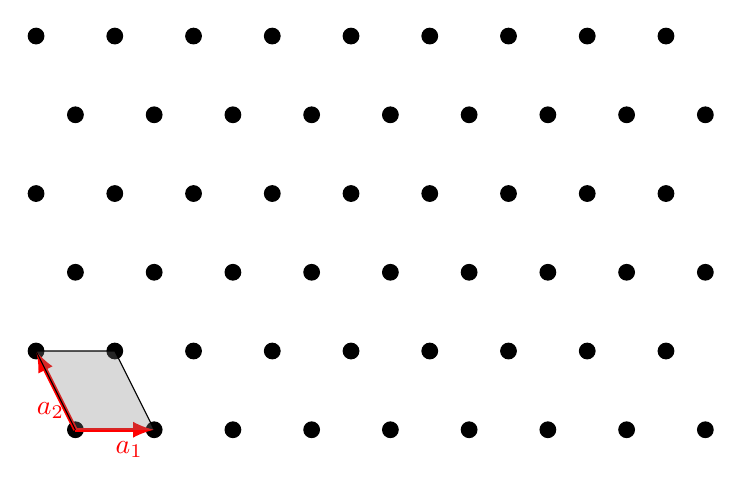
\begin{tikzpicture} 
          \foreach \y in {0,2,4}{
              \foreach \x in {1, 2, 3, 4, 5, 6, 7, 8, 9}{
                  \node[draw, circle, inner sep=2pt, fill] at (\x,\y){};
              }
          }
          \foreach \y in {1,3,5}{
              \foreach \x in {0.5, 1.5, 2.5, 3.5, 4.5, 5.5, 6.5, 7.5, 8.5}{
                  \node[draw, circle, inner sep=2pt, fill] at (\x,\y){};
              }
          }
          \draw [ultra thick, -latex, red] (1, 0) -- (2, 0) node [below left] {$a_1$};
          \draw [ultra thick, -latex, red]  (1, 0) node [above left] {$a_2$} -- (0.5, 1) ;
          \filldraw[fill=gray, fill opacity=0.3, draw=black] (1,0) -- (0.5,1) -- (1.5,1) -- (2,0);
          
      \end{tikzpicture}   
    \caption{lattice}
    \label{fig:hex}  
  \end{figure}
  %Draw reciprocal lattice
  \begin{figure}[ht]
    \centering
      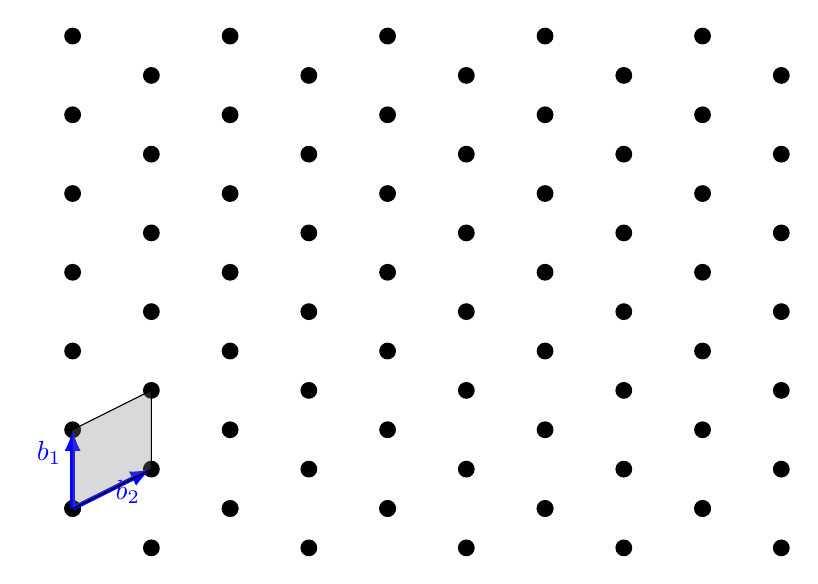
\begin{tikzpicture} 
          \foreach \x in {0,2,4,6,8}{
              \foreach \y in {1, 2, 3, 4, 5, 6, 7,}{
                  \node[draw, circle, inner sep=2pt, fill] at (\x,\y){};
              }
          }
          \foreach \x in {1,3,5,7,9}{
              \foreach \y in {0.5, 1.5, 2.5, 3.5, 4.5, 5.5, 6.5}{
                  \node[draw, circle, inner sep=2pt, fill] at (\x,\y){};
              }
          }
          \draw [ultra thick, -latex, blue] (0, 1) -- (0, 2) node [below left] {$b_1$};
          \draw [ultra thick, -latex, blue]  (0, 1) --  (1, 1.5) node [below left] {$b_2$} ;
          \filldraw[fill=gray, fill opacity=0.3, draw=black] (0,1) -- (1,1.5) -- (1,2.5) -- (0,2);
          
      \end{tikzpicture}   
    \caption{Reciprocal lattice}
    \label{fig:hex rep}  
  \end{figure}
Let us consider a general wave in the crystal
\begin{equation*}
    x_{u,v}(t) = u(0)\exp(-i\omega t)\exp(suk_1a)\exp(svk_2a)
\end{equation*}
Let us suppose that the last atom in the $\ve e_1$'s direction has coordinates $(Na,0)$ and the last one along $\ve e_2$ has coordinates $(0, Na)$ (or, in other words, let us suppose that we have $N$ atoms in each direction).
The boundary conditions are formally the same of the 2D's rectangular lattice, that is 
\begin{gather*}
    x_{0,v} = x_{N,v} \\
    x_{u,0} = x_{u,N}
\end{gather*}
hence the modes in the crystals are described by wavevectors $\ve k = (k_1, k_2)$ whose admitted values are for both
$$k_{s} = \frac{s\pi}{L} = \frac{s\pi}{Na}$$ 
where $N$ denotes the number of atoms in the crystal. The spacing (area) between two successive modes is the area of the unit cell
$\Delta k \equiv \frac{\sqrt{3}}{2} \frac{\pi^2}{L^2}$. The number of modes contained in a quarter of a circle of radius $k_0$ is given by 
\begin{equation*}
    n(k < k_0) = \frac{1}{4} \frac{\pi k_0^2}{\Delta k} = \frac{k_0^2 L^2}{2\sqrt{3}\,\pi}
\end{equation*}
The total number of modes of oscillation (degrees of fredom) is $2N$ where $N$ is the number of atoms. Hence the maximum allowed $k$ is 
\begin{equation*}
    k_D^2 = k_{max}^2 = \frac{2 \sqrt{3} \pi}{L^2} \, n = \frac{4 \sqrt{3} \pi}{L^2} \, N
\end{equation*}
and using the Debye's dispersion relation $\omega = v \, k$
\begin{equation*}
    \omega_D^2 = v^2 \frac{4 \sqrt{3} \pi }{L^2} \, N = \frac{4 \sqrt{3} \pi }{N a^2} \, v^2 
\end{equation*}
so that the Debye's frequency is 
\begin{equation*}
    \omega_D = \frac{2v}{a} \sqrt{\frac{\sqrt{3} \pi }{N}} \simeq 
\end{equation*}